\documentclass[a4paper]{book}
\usepackage{a4wide}
\usepackage{makeidx}
\usepackage{graphicx}
\usepackage{multicol}
\usepackage{float}
\usepackage{listings}
\usepackage{color}
\usepackage{textcomp}
\usepackage{alltt}
\usepackage{times}
\usepackage{ifpdf}
\ifpdf
\usepackage[pdftex,
            pagebackref=true,
            colorlinks=true,
            linkcolor=blue,
            unicode
           ]{hyperref}
\else
\usepackage[ps2pdf,
            pagebackref=true,
            colorlinks=true,
            linkcolor=blue,
            unicode
           ]{hyperref}
\usepackage{pspicture}
\fi
\usepackage[utf8]{inputenc}
\usepackage{doxygen}
\lstset{language=C++,inputencoding=utf8,basicstyle=\footnotesize,breaklines=true,breakatwhitespace=true,tabsize=8,numbers=left }
\makeindex
\setcounter{tocdepth}{3}
\renewcommand{\footrulewidth}{0.4pt}
\begin{document}
\hypersetup{pageanchor=false}
\begin{titlepage}
\vspace*{7cm}
\begin{center}
{\Large Arduino GLCD Library \\[1ex]\large 1 }\\
\vspace*{1cm}
{\large Generated by Doxygen 1.6.2}\\
\vspace*{0.5cm}
{\small Tue Jan 19 20:45:02 2010}\\
\end{center}
\end{titlepage}
\clearemptydoublepage
\pagenumbering{roman}
\tableofcontents
\clearemptydoublepage
\pagenumbering{arabic}
\hypersetup{pageanchor=true}
\chapter{Class Index}
\section{Class Hierarchy}
This inheritance list is sorted roughly, but not completely, alphabetically:\begin{DoxyCompactList}
\item \contentsline{section}{glcd\_\-Device}{\pageref{classglcd___device}}{}
\begin{DoxyCompactList}
\item \contentsline{section}{glcd}{\pageref{classglcd}}{}
\end{DoxyCompactList}
\item \contentsline{section}{gText}{\pageref{classg_text}}{}
\item \contentsline{section}{lcdCoord}{\pageref{structlcd_coord}}{}
\item \contentsline{section}{twin}{\pageref{structtwin}}{}
\item \contentsline{section}{twincntxt}{\pageref{structtwincntxt}}{}
\end{DoxyCompactList}

\chapter{Class Index}
\section{Class List}
Here are the classes, structs, unions and interfaces with brief descriptions:\begin{DoxyCompactList}
\item\contentsline{section}{\hyperlink{classglcd}{glcd} }{\pageref{classglcd}}{}
\item\contentsline{section}{\hyperlink{classglcd___device}{glcd\_\-Device} }{\pageref{classglcd___device}}{}
\item\contentsline{section}{\hyperlink{classg_text}{gText} }{\pageref{classg_text}}{}
\item\contentsline{section}{\hyperlink{structlcd_coord}{lcdCoord} }{\pageref{structlcd_coord}}{}
\item\contentsline{section}{\hyperlink{structtwin}{twin} }{\pageref{structtwin}}{}
\item\contentsline{section}{\hyperlink{structtwincntxt}{twincntxt} }{\pageref{structtwincntxt}}{}
\end{DoxyCompactList}

\chapter{Class Documentation}
\hypertarget{classglcd}{
\section{glcd Class Reference}
\label{classglcd}\index{glcd@{glcd}}
}
Inheritance diagram for glcd::\begin{figure}[H]
\begin{center}
\leavevmode
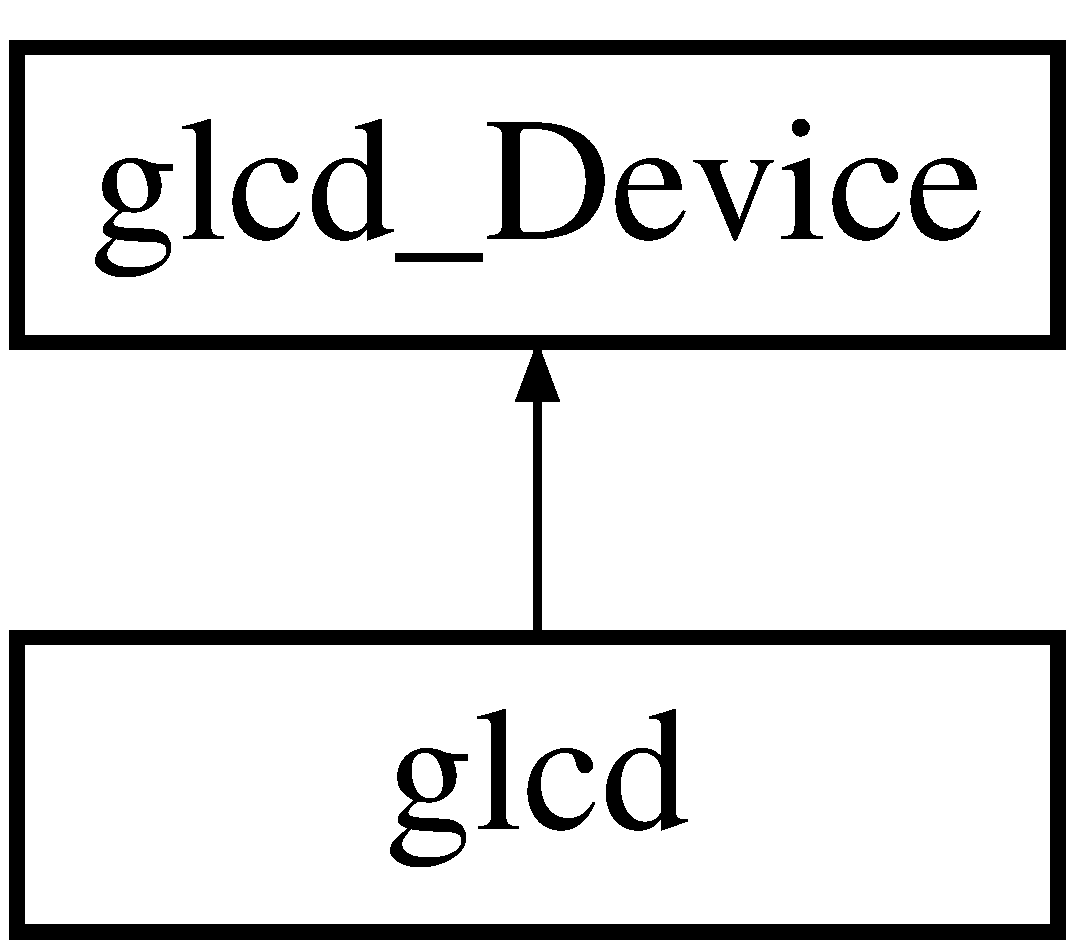
\includegraphics[height=2cm]{classglcd}
\end{center}
\end{figure}
\subsection*{Public Member Functions}
\begin{DoxyCompactItemize}
\item 
void \hyperlink{classglcd_aba75fe511781243aeb06df806bb4782a}{Init} (uint8\_\-t invert=NON\_\-INVERTED)
\item 
\hypertarget{classglcd_aee55835080cf4b713f98dbfc5b98af16}{
void {\bfseries ClearPage} (uint8\_\-t page, uint8\_\-t color=WHITE)}
\label{classglcd_aee55835080cf4b713f98dbfc5b98af16}

\item 
\hypertarget{classglcd_a1f3d55d537a3aa0932a9c0c2e08dab32}{
void {\bfseries ClearPage} (uint8\_\-t page, uint8\_\-t startX, uint8\_\-t length, uint8\_\-t color=WHITE)}
\label{classglcd_a1f3d55d537a3aa0932a9c0c2e08dab32}

\item 
void \hyperlink{classglcd_a0bfcbfcca05643356eefbc0f94a62ea6}{ClearScreen} (uint8\_\-t color=WHITE)
\item 
void \hyperlink{classglcd_a93adb4256767b495b15fb326d6d2c01a}{DrawVLine} (uint8\_\-t x, uint8\_\-t y, uint8\_\-t height, uint8\_\-t color=BLACK)
\item 
void \hyperlink{classglcd_ad44a983103e20535558b69ba15504493}{DrawHLine} (uint8\_\-t x, uint8\_\-t y, uint8\_\-t width, uint8\_\-t color=BLACK)
\item 
void \hyperlink{classglcd_a2995efe72f737e151794898d0f3f784f}{DrawLine} (uint8\_\-t x1, uint8\_\-t y1, uint8\_\-t x2, uint8\_\-t y2, uint8\_\-t color=BLACK)
\item 
void \hyperlink{classglcd_adbbbba35a6019a7b050e6234619446c0}{DrawRect} (uint8\_\-t x, uint8\_\-t y, uint8\_\-t width, uint8\_\-t height, uint8\_\-t color=BLACK)
\item 
\hypertarget{classglcd_a68b290c71c58892ac7092b72325db754}{
void {\bfseries DrawRoundRect} (uint8\_\-t x, uint8\_\-t y, uint8\_\-t width, uint8\_\-t height, uint8\_\-t radius, uint8\_\-t color=BLACK)}
\label{classglcd_a68b290c71c58892ac7092b72325db754}

\item 
void \hyperlink{classglcd_ac3ee3809429b633e17734b0b8ca7d010}{FillRect} (uint8\_\-t x, uint8\_\-t y, uint8\_\-t width, uint8\_\-t height, uint8\_\-t color=BLACK)
\item 
\hypertarget{classglcd_a09d544feba1fbe36b98b18cc3fa0c129}{
void {\bfseries InvertRect} (uint8\_\-t x, uint8\_\-t y, uint8\_\-t width, uint8\_\-t height)}
\label{classglcd_a09d544feba1fbe36b98b18cc3fa0c129}

\item 
\hypertarget{classglcd_a91c42301a5a8e808b59cbd6645500aed}{
void {\bfseries DrawCircle} (uint8\_\-t xCenter, uint8\_\-t yCenter, uint8\_\-t radius, uint8\_\-t color=BLACK)}
\label{classglcd_a91c42301a5a8e808b59cbd6645500aed}

\item 
\hypertarget{classglcd_a4c2f797be7a06cefbe38c818d5c81d14}{
void {\bfseries SetInverted} (uint8\_\-t invert)}
\label{classglcd_a4c2f797be7a06cefbe38c818d5c81d14}

\item 
\hypertarget{classglcd_ab908033b23619189d8cc2c54705f9893}{
void {\bfseries DrawBitmap} (const uint8\_\-t $\ast$bitmap, uint8\_\-t x, uint8\_\-t y, uint8\_\-t color=BLACK)}
\label{classglcd_ab908033b23619189d8cc2c54705f9893}

\item 
\hypertarget{classglcd_a774feb284411700450cc959ba95e019f}{
void {\bfseries SelectFont} (const uint8\_\-t $\ast$font, uint8\_\-t color=BLACK)}
\label{classglcd_a774feb284411700450cc959ba95e019f}

\item 
\hypertarget{classglcd_a0dac9c9863cc69b0b4ce722158f131a1}{
void {\bfseries Puts\_\-P} (PGM\_\-P str)}
\label{classglcd_a0dac9c9863cc69b0b4ce722158f131a1}

\item 
\hypertarget{classglcd_a3dbc964830f5004c4482a5f4045f90e8}{
int {\bfseries PutChar} (char c) \_\-\_\-attribute\_\-\_\-((deprecated))}
\label{classglcd_a3dbc964830f5004c4482a5f4045f90e8}

\item 
\hypertarget{classglcd_a19cb66c2aa302634345dedb6f9036243}{
void {\bfseries Puts} (char $\ast$str)}
\label{classglcd_a19cb66c2aa302634345dedb6f9036243}

\item 
\hypertarget{classglcd_a0343e2c770509d75cf19c38e0fec8d5f}{
{\bfseries \_\-\_\-attribute\_\-\_\-} ((deprecated))}
\label{classglcd_a0343e2c770509d75cf19c38e0fec8d5f}

\item 
\hypertarget{classglcd_a800dce3fee15490eb416d94688c2bca5}{
void {\bfseries PrintNumber} (long n)}
\label{classglcd_a800dce3fee15490eb416d94688c2bca5}

\item 
\hypertarget{classglcd_a0343e2c770509d75cf19c38e0fec8d5f}{
{\bfseries \_\-\_\-attribute\_\-\_\-} ((deprecated))}
\label{classglcd_a0343e2c770509d75cf19c38e0fec8d5f}

\item 
\hypertarget{classglcd_a26bc8c556e4c7bae32619b9f3cb733d8}{
void {\bfseries ClearSysTextLine} (uint8\_\-t row)}
\label{classglcd_a26bc8c556e4c7bae32619b9f3cb733d8}

\item 
\hypertarget{classglcd_a4aaa1849b81c34844cffa1cf01e37e39}{
void {\bfseries CursorTo} (uint8\_\-t column, uint8\_\-t row)}
\label{classglcd_a4aaa1849b81c34844cffa1cf01e37e39}

\item 
\hypertarget{classglcd_afd6683a3a20254d57a3ddc2069cbb18d}{
void {\bfseries write} (uint8\_\-t c)}
\label{classglcd_afd6683a3a20254d57a3ddc2069cbb18d}

\item 
\hypertarget{classglcd_a7329a9661c9d38f4c221c70f7c867e24}{
uint8\_\-t {\bfseries CharWidth} (char c)}
\label{classglcd_a7329a9661c9d38f4c221c70f7c867e24}

\item 
\hypertarget{classglcd_a4b9e13b6ab8d3fad24f71fc32ff40a82}{
uint16\_\-t {\bfseries StringWidth} (const char $\ast$str)}
\label{classglcd_a4b9e13b6ab8d3fad24f71fc32ff40a82}

\item 
\hypertarget{classglcd_a4066f4d5c02e422056da92d6b90d224b}{
uint16\_\-t {\bfseries StringWidth\_\-P} (PGM\_\-P str)}
\label{classglcd_a4066f4d5c02e422056da92d6b90d224b}

\end{DoxyCompactItemize}
\subsection*{Public Attributes}
\begin{DoxyCompactItemize}
\item 
\hypertarget{classglcd_a74a050a4cd0f4660fbcf3b8d79b3cd73}{
\hyperlink{classg_text}{gText} {\bfseries Text}}
\label{classglcd_a74a050a4cd0f4660fbcf3b8d79b3cd73}

\end{DoxyCompactItemize}
\subsection*{Static Public Attributes}
\begin{DoxyCompactItemize}
\item 
\hypertarget{classglcd_ade27e0efd44c425139650e4d455b1902}{
static const uint8\_\-t {\bfseries Width} = DISPLAY\_\-WIDTH}
\label{classglcd_ade27e0efd44c425139650e4d455b1902}

\item 
\hypertarget{classglcd_a5c39b5959eb3298731f6dfb22aec50d9}{
static const uint8\_\-t {\bfseries Height} = DISPLAY\_\-HEIGHT}
\label{classglcd_a5c39b5959eb3298731f6dfb22aec50d9}

\end{DoxyCompactItemize}


\subsection{Member Function Documentation}
\hypertarget{classglcd_a0bfcbfcca05643356eefbc0f94a62ea6}{
\index{glcd@{glcd}!ClearScreen@{ClearScreen}}
\index{ClearScreen@{ClearScreen}!glcd@{glcd}}
\subsubsection[{ClearScreen}]{\setlength{\rightskip}{0pt plus 5cm}void glcd::ClearScreen (uint8\_\-t {\em color} = {\ttfamily WHITE})}}
\label{classglcd_a0bfcbfcca05643356eefbc0f94a62ea6}
Clear the lcd display


\begin{DoxyParams}{Parameters}
\item[{\em color}]BLACK or WHITE\end{DoxyParams}
Sets all the pixels on the display from 0,0 to GLCD.Width-\/1,GLCD.Height-\/1 to the specified color.

Color is optional and defaults to WHITE.

\begin{DoxyNote}{Note}
If the display is in INVERTED mode, then the color WHITE will paint the screen BLACK and the color BLACK will paint the screen WHITE. 
\end{DoxyNote}
\hypertarget{classglcd_ad44a983103e20535558b69ba15504493}{
\index{glcd@{glcd}!DrawHLine@{DrawHLine}}
\index{DrawHLine@{DrawHLine}!glcd@{glcd}}
\subsubsection[{DrawHLine}]{\setlength{\rightskip}{0pt plus 5cm}void glcd::DrawHLine (uint8\_\-t {\em x}, \/  uint8\_\-t {\em y}, \/  uint8\_\-t {\em width}, \/  uint8\_\-t {\em color} = {\ttfamily BLACK})}}
\label{classglcd_ad44a983103e20535558b69ba15504493}
Draw a Horizontal Line


\begin{DoxyParams}{Parameters}
\item[{\em x}]a value from 0 to GLCD.Width-\/1 \item[{\em y}]a value from 0 to GLCD.Height-\/1 \item[{\em width}]a value from 1 to GLCD.Width-\/x-\/1 \item[{\em color}]BLACK or WHITE\end{DoxyParams}
The line drawn will be width+1 pixels.

color is an optional parameter indicating pixel color and defaults to BLACK

\begin{DoxyNote}{Note}
This function was previously named DrawHoriLine() in the ks0108 library
\end{DoxyNote}
\begin{DoxySeeAlso}{See also}
\hyperlink{classglcd_a2995efe72f737e151794898d0f3f784f}{DrawLine()} 

\hyperlink{classglcd_a93adb4256767b495b15fb326d6d2c01a}{DrawVLine()} 
\end{DoxySeeAlso}
\hypertarget{classglcd_a2995efe72f737e151794898d0f3f784f}{
\index{glcd@{glcd}!DrawLine@{DrawLine}}
\index{DrawLine@{DrawLine}!glcd@{glcd}}
\subsubsection[{DrawLine}]{\setlength{\rightskip}{0pt plus 5cm}void glcd::DrawLine (uint8\_\-t {\em x1}, \/  uint8\_\-t {\em y1}, \/  uint8\_\-t {\em x2}, \/  uint8\_\-t {\em y2}, \/  uint8\_\-t {\em color} = {\ttfamily BLACK})}}
\label{classglcd_a2995efe72f737e151794898d0f3f784f}
Draw a line


\begin{DoxyParams}{Parameters}
\item[{\em x1}]a value from 0 to GLCD.Width-\/1 indicating start x coordinate \item[{\em y1}]a value fron 0 to GLCD.Height-\/1 indicating start y coordinate \item[{\em x2}]a value from 0 to GLCD.Width-\/1 indicating end x coordinate \item[{\em y2}]a value fron 0 to GLCD.Height-\/1 indicating end y coordinate \item[{\em color}]BLACK or WHITE\end{DoxyParams}
Draws a line starting at x1,y2 and ending at x2,y2.

Color is optional and defaults to BLACK.

\begin{DoxySeeAlso}{See also}
\hyperlink{classglcd_ad44a983103e20535558b69ba15504493}{DrawHLine()} 

\hyperlink{classglcd_a93adb4256767b495b15fb326d6d2c01a}{DrawVLine()} 
\end{DoxySeeAlso}
\hypertarget{classglcd_adbbbba35a6019a7b050e6234619446c0}{
\index{glcd@{glcd}!DrawRect@{DrawRect}}
\index{DrawRect@{DrawRect}!glcd@{glcd}}
\subsubsection[{DrawRect}]{\setlength{\rightskip}{0pt plus 5cm}void glcd::DrawRect (uint8\_\-t {\em x}, \/  uint8\_\-t {\em y}, \/  uint8\_\-t {\em width}, \/  uint8\_\-t {\em height}, \/  uint8\_\-t {\em color} = {\ttfamily BLACK})}}
\label{classglcd_adbbbba35a6019a7b050e6234619446c0}
Draw a rectangle of given width and height


\begin{DoxyParams}{Parameters}
\item[{\em x}]the x coordinate of the upper left corner of the rectangle \item[{\em y}]the y coordinate of the upper left corner of the rectangle \item[{\em width}]width of the rectangle \item[{\em height}]height of the rectangle \item[{\em color}]BLACK or WHITE\end{DoxyParams}
Draws a rectangle with the specified width and height. The upper left corner at x,y and the lower right corner at x+width,y+width.

The length of the horizontal sides will be width+1 pixels The length of the vertical sides will be height+1 pixels

Color is optional and defaults to BLACK.

\begin{DoxyNote}{Note}
The width and height parameters work differently than \hyperlink{classglcd_ac3ee3809429b633e17734b0b8ca7d010}{FillRect()}
\end{DoxyNote}
\begin{DoxySeeAlso}{See also}
\hyperlink{classglcd_ac3ee3809429b633e17734b0b8ca7d010}{FillRect()} 
\end{DoxySeeAlso}
\hypertarget{classglcd_a93adb4256767b495b15fb326d6d2c01a}{
\index{glcd@{glcd}!DrawVLine@{DrawVLine}}
\index{DrawVLine@{DrawVLine}!glcd@{glcd}}
\subsubsection[{DrawVLine}]{\setlength{\rightskip}{0pt plus 5cm}void glcd::DrawVLine (uint8\_\-t {\em x}, \/  uint8\_\-t {\em y}, \/  uint8\_\-t {\em height}, \/  uint8\_\-t {\em color} = {\ttfamily BLACK})}}
\label{classglcd_a93adb4256767b495b15fb326d6d2c01a}
Draw a Vertical Line


\begin{DoxyParams}{Parameters}
\item[{\em x}]a value from 0 to GLCD.Width-\/1 \item[{\em y}]a value from 0 to GLCD.Height-\/1 \item[{\em height}]a value from 1 to GLCD.Height-\/y-\/1\end{DoxyParams}
BLACK or WHITE is an optional parameter indicating pixel color, default is BLACK

The line drawn will be height+1 pixels.

\begin{DoxyNote}{Note}
This function was previously named DrawVertLine() in the ks0108 library
\end{DoxyNote}
\begin{DoxySeeAlso}{See also}
\hyperlink{classglcd_a2995efe72f737e151794898d0f3f784f}{DrawLine()} 

\hyperlink{classglcd_ad44a983103e20535558b69ba15504493}{DrawHLine()} 
\end{DoxySeeAlso}
\hypertarget{classglcd_ac3ee3809429b633e17734b0b8ca7d010}{
\index{glcd@{glcd}!FillRect@{FillRect}}
\index{FillRect@{FillRect}!glcd@{glcd}}
\subsubsection[{FillRect}]{\setlength{\rightskip}{0pt plus 5cm}void glcd::FillRect (uint8\_\-t {\em x}, \/  uint8\_\-t {\em y}, \/  uint8\_\-t {\em width}, \/  uint8\_\-t {\em height}, \/  uint8\_\-t {\em color} = {\ttfamily BLACK})}}
\label{classglcd_ac3ee3809429b633e17734b0b8ca7d010}
Fill a Rectangle


\begin{DoxyParams}{Parameters}
\item[{\em x}]the x coordinate of the upper left corner of the rectangle \item[{\em y}]the y coordinate of the upper left corner of the rectangle \item[{\em width}]width of the rectangle \item[{\em height}]height of the rectangle \item[{\em color}]BLACK or WHITE\end{DoxyParams}
Fills a rectanglular area of the specified width and height.

The resulting rectangle covers an area width pixels wide by height pixels tall starting from the pixel at x,y.

The upper left corner at x,y and the lower right corner at x+width-\/1,y+width-\/1.

The length of the horizontal sides will be width pixels The length of the vertical sides will be height pixels

Color is optional and defaults to BLACK.

\begin{DoxyNote}{Note}
The width and height parameters work differently than \hyperlink{classglcd_adbbbba35a6019a7b050e6234619446c0}{DrawRect()}
\end{DoxyNote}
\begin{DoxyWarning}{Warning}
\hyperlink{classglcd_ac3ee3809429b633e17734b0b8ca7d010}{FillRect()} behavior has changed from the previous versions of the ks0108 library. The filled rectangle will be one pixel smaller in width and height than the old version. This change was to make the functionality consistent with the way Java and C\# create filled rectangles
\end{DoxyWarning}
\begin{DoxySeeAlso}{See also}
\hyperlink{classglcd_adbbbba35a6019a7b050e6234619446c0}{DrawRect()} 
\end{DoxySeeAlso}
\hypertarget{classglcd_aba75fe511781243aeb06df806bb4782a}{
\index{glcd@{glcd}!Init@{Init}}
\index{Init@{Init}!glcd@{glcd}}
\subsubsection[{Init}]{\setlength{\rightskip}{0pt plus 5cm}void glcd::Init (uint8\_\-t {\em invert} = {\ttfamily NON\_\-INVERTED})}}
\label{classglcd_aba75fe511781243aeb06df806bb4782a}
Initilize the GLCD library and hardware


\begin{DoxyParams}{Parameters}
\item[{\em invert}]specifices whether display is in normal mode or inverted mode.\end{DoxyParams}
This should be called prior to any other graphic library function. It does all the needed initializations including taking care of the low level hardware initalization of the display device.

The optional invert parameter specifies if the display should be run in a normal mode, dark pixels on light background or inverted, light pixels on a dark background.

To specify dark pixels use the define {\bfseries NON-\/INVERTED} and to use light pixels use the define {\bfseries INVERTED} 

Upon completion of the initialization, then entire display will be cleared. 

Reimplemented from \hyperlink{classglcd___device_a15bd97b27644f9962f2e50a442b4cdcc}{glcd\_\-Device}.

The documentation for this class was generated from the following files:\begin{DoxyCompactItemize}
\item 
C:/Users/bill/Documents/000-\/NewHomeDir/My-\/Documents/Scuba-\/Stuff/Aeris/Download-\/Protocol/devel/windows/arduino-\/0017/hardware/libraries/glcd/glcd.h\item 
C:/Users/bill/Documents/000-\/NewHomeDir/My-\/Documents/Scuba-\/Stuff/Aeris/Download-\/Protocol/devel/windows/arduino-\/0017/hardware/libraries/glcd/glcd.cpp\end{DoxyCompactItemize}

\hypertarget{classglcd___device}{
\section{glcd\_\-Device Class Reference}
\label{classglcd___device}\index{glcd\_\-Device@{glcd\_\-Device}}
}
Inheritance diagram for glcd\_\-Device::\begin{figure}[H]
\begin{center}
\leavevmode
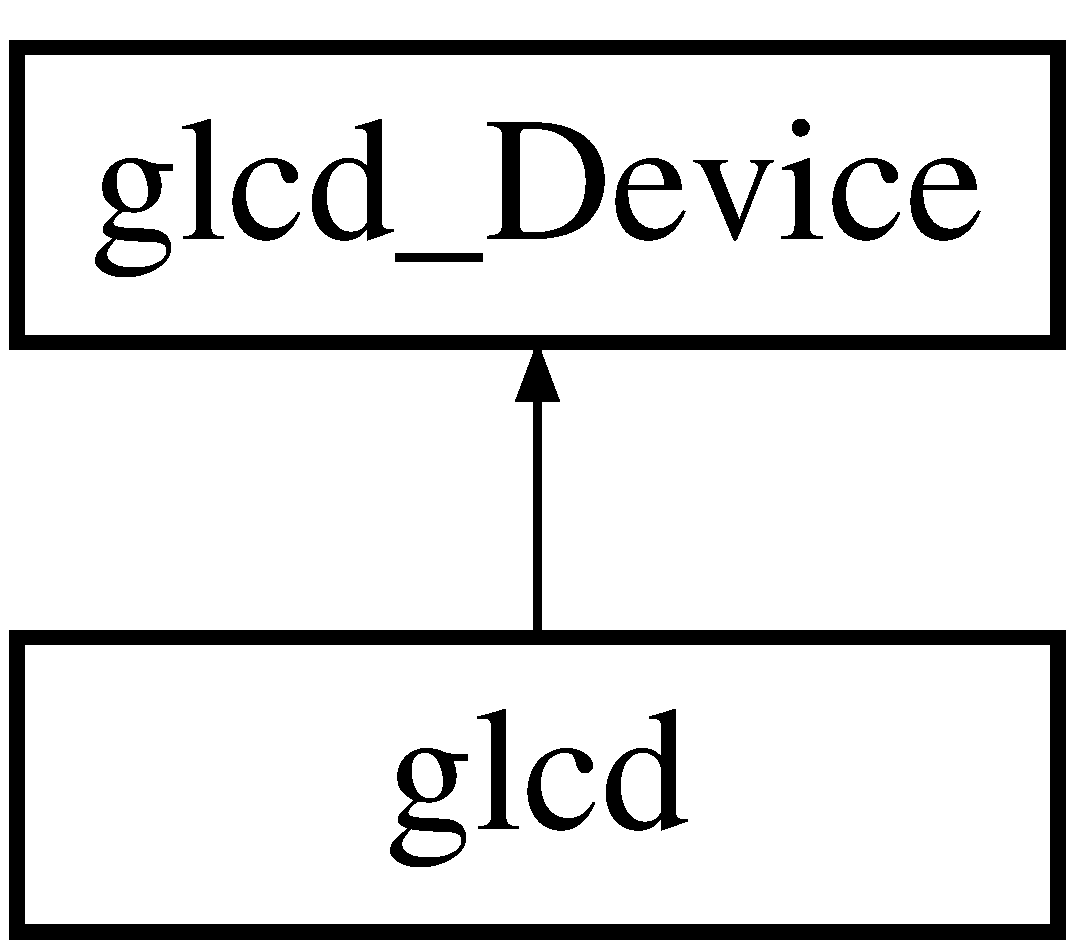
\includegraphics[height=2cm]{classglcd___device}
\end{center}
\end{figure}
\subsection*{Public Member Functions}
\begin{DoxyCompactItemize}
\item 
void \hyperlink{classglcd___device_a15bd97b27644f9962f2e50a442b4cdcc}{Init} (uint8\_\-t invert)
\item 
void \hyperlink{classglcd___device_ad5fd910ef008e2d04e8d9b4fd8cac543}{GotoXY} (uint8\_\-t x, uint8\_\-t y)
\item 
void \hyperlink{classglcd___device_a1916258e850cd839172ce318a0b903fd}{SetDot} (uint8\_\-t x, uint8\_\-t y, uint8\_\-t color)
\item 
void \hyperlink{classglcd___device_a4950fe109b27cb1cdcdbabe367d02c80}{SetPixels} (uint8\_\-t x, uint8\_\-t y, uint8\_\-t x1, uint8\_\-t y1, uint8\_\-t color)
\item 
uint8\_\-t \hyperlink{classglcd___device_a2ec1756ae0c7787fad676d6398c73de3}{ReadData} (void)
\item 
void \hyperlink{classglcd___device_a209d1ba245e7e02eb65e07c15ce0461d}{WriteData} (uint8\_\-t data)
\end{DoxyCompactItemize}
\subsection*{Public Attributes}
\begin{DoxyCompactItemize}
\item 
\hypertarget{classglcd___device_a553e9a639bfbf4f971d90ea0846f2882}{
uint8\_\-t {\bfseries Inverted}}
\label{classglcd___device_a553e9a639bfbf4f971d90ea0846f2882}

\item 
\hypertarget{classglcd___device_a72748fb53a38a2d471ed46bf3a22e698}{
\hyperlink{structlcd_coord}{lcdCoord} {\bfseries Coord}}
\label{classglcd___device_a72748fb53a38a2d471ed46bf3a22e698}

\end{DoxyCompactItemize}


\subsection{Member Function Documentation}
\hypertarget{classglcd___device_ad5fd910ef008e2d04e8d9b4fd8cac543}{
\index{glcd\_\-Device@{glcd\_\-Device}!GotoXY@{GotoXY}}
\index{GotoXY@{GotoXY}!glcd_Device@{glcd\_\-Device}}
\subsubsection[{GotoXY}]{\setlength{\rightskip}{0pt plus 5cm}void glcd\_\-Device::GotoXY (uint8\_\-t {\em x}, \/  uint8\_\-t {\em y})}}
\label{classglcd___device_ad5fd910ef008e2d04e8d9b4fd8cac543}
set current x,y coordinate on display device


\begin{DoxyParams}{Parameters}
\item[{\em x}]X coordinate \item[{\em y}]Y coordinate\end{DoxyParams}
Sets the current pixel location to x,y. x and y are relative to the 0,0 origin of the display which is the upper left most pixel on the display. \hypertarget{classglcd___device_a15bd97b27644f9962f2e50a442b4cdcc}{
\index{glcd\_\-Device@{glcd\_\-Device}!Init@{Init}}
\index{Init@{Init}!glcd_Device@{glcd\_\-Device}}
\subsubsection[{Init}]{\setlength{\rightskip}{0pt plus 5cm}void glcd\_\-Device::Init (uint8\_\-t {\em invert})}}
\label{classglcd___device_a15bd97b27644f9962f2e50a442b4cdcc}
Low level h/w initialization of display and AVR pins


\begin{DoxyParams}{Parameters}
\item[{\em invert}]specifices whether display is in normal mode or inverted mode.\end{DoxyParams}
This should only be called prior by other library code.

It does all the low level hardware initalization of the display device.

The optional invert parameter specifies if the display should be run in a normal mode, dark pixels on light background or inverted, light pixels on a dark background.

To specify dark pixels use the define {\bfseries NON-\/INVERTED} and to use light pixels use the define {\bfseries INVERTED} 

Upon completion of the initialization, then entire display will be cleared. 

Reimplemented in \hyperlink{classglcd_aba75fe511781243aeb06df806bb4782a}{glcd}.\hypertarget{classglcd___device_a2ec1756ae0c7787fad676d6398c73de3}{
\index{glcd\_\-Device@{glcd\_\-Device}!ReadData@{ReadData}}
\index{ReadData@{ReadData}!glcd_Device@{glcd\_\-Device}}
\subsubsection[{ReadData}]{\setlength{\rightskip}{0pt plus 5cm}uint8\_\-t glcd\_\-Device::ReadData (void)\hspace{0.3cm}{\ttfamily  \mbox{[}inline\mbox{]}}}}
\label{classglcd___device_a2ec1756ae0c7787fad676d6398c73de3}
read a data byte from display device memory

\begin{DoxyReturn}{Returns}
the data byte at the current x,y position
\end{DoxyReturn}
\begin{DoxyNote}{Note}
the current x,y location is not modified by the routine. This allows a read/modify/write operation. Code can call \hyperlink{classglcd___device_a2ec1756ae0c7787fad676d6398c73de3}{ReadData()} modify the data then call \hyperlink{classglcd___device_a209d1ba245e7e02eb65e07c15ce0461d}{WriteData()} and update the same location.
\end{DoxyNote}
\begin{DoxySeeAlso}{See also}
\hyperlink{classglcd___device_a209d1ba245e7e02eb65e07c15ce0461d}{WriteData()} 
\end{DoxySeeAlso}
\hypertarget{classglcd___device_a1916258e850cd839172ce318a0b903fd}{
\index{glcd\_\-Device@{glcd\_\-Device}!SetDot@{SetDot}}
\index{SetDot@{SetDot}!glcd_Device@{glcd\_\-Device}}
\subsubsection[{SetDot}]{\setlength{\rightskip}{0pt plus 5cm}void glcd\_\-Device::SetDot (uint8\_\-t {\em x}, \/  uint8\_\-t {\em y}, \/  uint8\_\-t {\em color})}}
\label{classglcd___device_a1916258e850cd839172ce318a0b903fd}
set pixel at x,y to the given color


\begin{DoxyParams}{Parameters}
\item[{\em x}]X coordinate \item[{\em y}]Y coordinate \item[{\em color}]WHITE or BLACK\end{DoxyParams}
Sets the pixel at location x,y to the specified color. x and y are relative to the 0,0 origin of the display which is the upper left corner.

\begin{DoxyNote}{Note}
If the display has been set to INVERTED mode then the colors will be automically reversed. 
\end{DoxyNote}
\hypertarget{classglcd___device_a4950fe109b27cb1cdcdbabe367d02c80}{
\index{glcd\_\-Device@{glcd\_\-Device}!SetPixels@{SetPixels}}
\index{SetPixels@{SetPixels}!glcd_Device@{glcd\_\-Device}}
\subsubsection[{SetPixels}]{\setlength{\rightskip}{0pt plus 5cm}void glcd\_\-Device::SetPixels (uint8\_\-t {\em x}, \/  uint8\_\-t {\em y}, \/  uint8\_\-t {\em x2}, \/  uint8\_\-t {\em y2}, \/  uint8\_\-t {\em color})}}
\label{classglcd___device_a4950fe109b27cb1cdcdbabe367d02c80}
set an area of pixels


\begin{DoxyParams}{Parameters}
\item[{\em x}]X coordinate of upper left corner \item[{\em y}]Y coordinate of upper left corner \item[{\em x2}]X coordinate of lower right corner \item[{\em y2}]Y coordinate of lower right corner\end{DoxyParams}
sets the pixels an area bounded by x,y to x2,y2 inclusive to the specified color.

The width of the area is x2-\/x + 1. The height of the area is y2-\/y+1 \hypertarget{classglcd___device_a209d1ba245e7e02eb65e07c15ce0461d}{
\index{glcd\_\-Device@{glcd\_\-Device}!WriteData@{WriteData}}
\index{WriteData@{WriteData}!glcd_Device@{glcd\_\-Device}}
\subsubsection[{WriteData}]{\setlength{\rightskip}{0pt plus 5cm}void glcd\_\-Device::WriteData (uint8\_\-t {\em data})}}
\label{classglcd___device_a209d1ba245e7e02eb65e07c15ce0461d}
Write a byte to display device memory


\begin{DoxyParams}{Parameters}
\item[{\em data}]date byte to write to memory\end{DoxyParams}
The data specified is written to glcd memory at the current x,y position. If the y location is not on a byte boundary, the write is fragemented up into multiple writes.

\begin{DoxyNote}{Note}
the full behavior of this during split byte writes currently varies depending on a compile time define. The code can be configured to either OR in 1 data bits or set all the data bits. {\bfseries TRUE\_\-WRITE} controls this behavior.

the x,y address will not be the same as it was prior to this call. The y address will remain the aame but the x address will advance by one. This allows back to writes to write sequentially through memory without having to do additional x,y positioning.
\end{DoxyNote}
\begin{DoxySeeAlso}{See also}
\hyperlink{classglcd___device_a2ec1756ae0c7787fad676d6398c73de3}{ReadData()} 
\end{DoxySeeAlso}


The documentation for this class was generated from the following files:\begin{DoxyCompactItemize}
\item 
C:/Users/bill/Documents/000-\/NewHomeDir/My-\/Documents/Scuba-\/Stuff/Aeris/Download-\/Protocol/devel/windows/arduino-\/0017/hardware/libraries/glcd/glcd\_\-Device.h\item 
C:/Users/bill/Documents/000-\/NewHomeDir/My-\/Documents/Scuba-\/Stuff/Aeris/Download-\/Protocol/devel/windows/arduino-\/0017/hardware/libraries/glcd/glcd\_\-Device.cpp\end{DoxyCompactItemize}

\hypertarget{classg_text}{
\section{gText Class Reference}
\label{classg_text}\index{gText@{gText}}
}
\subsection*{Public Member Functions}
\begin{DoxyCompactItemize}
\item 
\hypertarget{classg_text_a41b4390adf51c17094b40fa1080ccc7c}{
void {\bfseries Init} (\hyperlink{classglcd___device}{glcd\_\-Device} $\ast$\_\-device)}
\label{classg_text_a41b4390adf51c17094b40fa1080ccc7c}

\item 
void \hyperlink{classg_text_a8bc94b15c7864ef34491e8ef5681bfd4}{DefineArea} (uint8\_\-t x1, uint8\_\-t y1, uint8\_\-t x2, uint8\_\-t y2, int8\_\-t scrolldir=1)
\item 
void \hyperlink{classg_text_a99a194bcdd6f57e27752da45a8cf4a86}{DefineArea} (uint8\_\-t x1, uint8\_\-t y1, uint8\_\-t columns, uint8\_\-t rows, const uint8\_\-t $\ast$font, int8\_\-t scrolldir=1)
\item 
void \hyperlink{classg_text_a8918c2e7b5b1121a6c9051db049c85bf}{ClearArea} (void)
\item 
void \hyperlink{classg_text_a3d2fcd1f48b1e44611b7cf6fb2bae5db}{SelectArea} (uint8\_\-t area)
\item 
void \hyperlink{classg_text_a400107517f9f5fa106b692d1c15165d0}{SelectFont} (const uint8\_\-t $\ast$font, uint8\_\-t color=BLACK, FontCallback callback=ReadPgmData)
\item 
int \hyperlink{classg_text_a368fbed0d50735647595f2d12cbe167c}{PutChar} (char c)
\item 
void \hyperlink{classg_text_a7f537bfce982c46779f61321df66b018}{write} (uint8\_\-t c)
\item 
void \hyperlink{classg_text_a7ce5b6e29b0d26d85064e6235927af75}{CursorTo} (uint8\_\-t column, uint8\_\-t row)
\item 
void \hyperlink{classg_text_a299ea80c33b47ffc1043e472d48d670d}{CursorToXY} (uint8\_\-t x, uint8\_\-t y)
\item 
uint8\_\-t \hyperlink{classg_text_a6cb49e22a690752ea439e2773ae31ec1}{CharWidth} (char c)
\item 
uint16\_\-t \hyperlink{classg_text_a0dce9ad4c40e0d8b0487f4d2303bd8ef}{StringWidth} (const char $\ast$str)
\item 
uint16\_\-t \hyperlink{classg_text_ae6f8d92ff8240dee9e32f74b1cbff44a}{StringWidth\_\-P} (PGM\_\-P str)
\item 
\hypertarget{classg_text_a0012b4b875489197faba124f8670b68a}{
void {\bfseries ClearSysTextLine} (uint8\_\-t row)}
\label{classg_text_a0012b4b875489197faba124f8670b68a}

\end{DoxyCompactItemize}
\subsection*{Static Public Attributes}
\begin{DoxyCompactItemize}
\item 
\hypertarget{classg_text_a4b49a135fda410b98469a0a8c9d8fd25}{
static const uint8\_\-t {\bfseries AreaCount} = GLCD\_\-TAREA\_\-CNT}
\label{classg_text_a4b49a135fda410b98469a0a8c9d8fd25}

\end{DoxyCompactItemize}


\subsection{Member Function Documentation}
\hypertarget{classg_text_a6cb49e22a690752ea439e2773ae31ec1}{
\index{gText@{gText}!CharWidth@{CharWidth}}
\index{CharWidth@{CharWidth}!gText@{gText}}
\subsubsection[{CharWidth}]{\setlength{\rightskip}{0pt plus 5cm}uint8\_\-t gText::CharWidth (char {\em c})}}
\label{classg_text_a6cb49e22a690752ea439e2773ae31ec1}
Returns the pixel width of a character


\begin{DoxyParams}{Parameters}
\item[{\em c}]character to be sized\end{DoxyParams}
\begin{DoxyReturn}{Returns}
The width in pixels of the given character including any inter-\/character gap pixels following the character when the character is rendered on the display.
\end{DoxyReturn}
\begin{DoxyNote}{Note}
The font for the character is the font of the currently selected text area.
\end{DoxyNote}
\begin{DoxySeeAlso}{See also}
\hyperlink{classg_text_a0dce9ad4c40e0d8b0487f4d2303bd8ef}{StringWidth()} 

\hyperlink{classg_text_ae6f8d92ff8240dee9e32f74b1cbff44a}{StringWidth\_\-P()} 
\end{DoxySeeAlso}
\hypertarget{classg_text_a8918c2e7b5b1121a6c9051db049c85bf}{
\index{gText@{gText}!ClearArea@{ClearArea}}
\index{ClearArea@{ClearArea}!gText@{gText}}
\subsubsection[{ClearArea}]{\setlength{\rightskip}{0pt plus 5cm}void gText::ClearArea (void)}}
\label{classg_text_a8918c2e7b5b1121a6c9051db049c85bf}
Clear the active text area with the current font background color and home the cursor to upper left corner.

\begin{DoxySeeAlso}{See also}
\hyperlink{classg_text_a8bc94b15c7864ef34491e8ef5681bfd4}{DefineArea()} 

\hyperlink{classg_text_a3d2fcd1f48b1e44611b7cf6fb2bae5db}{SelectArea()} 
\end{DoxySeeAlso}
\hypertarget{classg_text_a7ce5b6e29b0d26d85064e6235927af75}{
\index{gText@{gText}!CursorTo@{CursorTo}}
\index{CursorTo@{CursorTo}!gText@{gText}}
\subsubsection[{CursorTo}]{\setlength{\rightskip}{0pt plus 5cm}void gText::CursorTo (uint8\_\-t {\em column}, \/  uint8\_\-t {\em row})}}
\label{classg_text_a7ce5b6e29b0d26d85064e6235927af75}
Positions cursor to a character based column and row.


\begin{DoxyParams}{Parameters}
\item[{\em column}]specifies the horizontal position \item[{\em row}]specifies the vertical position\end{DoxyParams}
Column and Row are zero based character positions and are relative the the upper left corner of the currently selected text area base on the size of the currently selected font.

While intended for fixed width fonts, positioning will work for variable width fonts.

When variable width fonts are used, the column is based on assuming a width of the widest character.

\begin{DoxySeeAlso}{See also}
\hyperlink{classg_text_a299ea80c33b47ffc1043e472d48d670d}{CursorToXY()} 
\end{DoxySeeAlso}
\hypertarget{classg_text_a299ea80c33b47ffc1043e472d48d670d}{
\index{gText@{gText}!CursorToXY@{CursorToXY}}
\index{CursorToXY@{CursorToXY}!gText@{gText}}
\subsubsection[{CursorToXY}]{\setlength{\rightskip}{0pt plus 5cm}void gText::CursorToXY (uint8\_\-t {\em x}, \/  uint8\_\-t {\em y})}}
\label{classg_text_a299ea80c33b47ffc1043e472d48d670d}
Positions cursor to a X,Y position


\begin{DoxyParams}{Parameters}
\item[{\em x}]specifies the horizontal locaion \item[{\em y}]specifies the vertical locaion\end{DoxyParams}
X \& Y are zero based pixel coordinates and are relative to the upper left corner of the currently selected text area.

\begin{DoxySeeAlso}{See also}
\hyperlink{classg_text_a7ce5b6e29b0d26d85064e6235927af75}{CursorTo()} 
\end{DoxySeeAlso}
\hypertarget{classg_text_a99a194bcdd6f57e27752da45a8cf4a86}{
\index{gText@{gText}!DefineArea@{DefineArea}}
\index{DefineArea@{DefineArea}!gText@{gText}}
\subsubsection[{DefineArea}]{\setlength{\rightskip}{0pt plus 5cm}void gText::DefineArea (uint8\_\-t {\em x}, \/  uint8\_\-t {\em y}, \/  uint8\_\-t {\em columns}, \/  uint8\_\-t {\em rows}, \/  const uint8\_\-t $\ast$ {\em font}, \/  int8\_\-t {\em scrolldir} = {\ttfamily 1})}}
\label{classg_text_a99a194bcdd6f57e27752da45a8cf4a86}
Define a Text area by columns and rows


\begin{DoxyParams}{Parameters}
\item[{\em x}]X coordinate of upper left corner \item[{\em y}]Y coordinate of upper left corner \item[{\em colums}]number of text columns \item[{\em rows}]number of text rows \item[{\em font}]a pointer defined in a font defintion file \item[{\em scrolldir}]$<$0 it scrolls down/reverse, $>$0 up/normal\end{DoxyParams}
Defines a text area sized to hold columns characters across and rows characters tall. It is properly sized for the specified font.

While intended for fixed width fonts, sizing will work for variable width fonts.

When variable width fonts are used, the column is based on assuming a width of the widest character.

x,y is an absolute coordinate and is relateive to the 0,0 origin of the display.

scrolldir is an optional parameter and defaults to normal/up

\begin{DoxyNote}{Note}
Upon creation of the text area, the cursor position for the text area will be set to x,y
\end{DoxyNote}
\begin{DoxySeeAlso}{See also}
\hyperlink{classg_text_a8918c2e7b5b1121a6c9051db049c85bf}{ClearArea()} 

\hyperlink{classg_text_a3d2fcd1f48b1e44611b7cf6fb2bae5db}{SelectArea()} 
\end{DoxySeeAlso}
\hypertarget{classg_text_a8bc94b15c7864ef34491e8ef5681bfd4}{
\index{gText@{gText}!DefineArea@{DefineArea}}
\index{DefineArea@{DefineArea}!gText@{gText}}
\subsubsection[{DefineArea}]{\setlength{\rightskip}{0pt plus 5cm}void gText::DefineArea (uint8\_\-t {\em x1}, \/  uint8\_\-t {\em y1}, \/  uint8\_\-t {\em x2}, \/  uint8\_\-t {\em y2}, \/  int8\_\-t {\em scrolldir} = {\ttfamily 1})}}
\label{classg_text_a8bc94b15c7864ef34491e8ef5681bfd4}
Define a text area by abolute coordinates


\begin{DoxyParams}{Parameters}
\item[{\em x1}]X coordinate of upper left corner \item[{\em y1}]Y coordinate of upper left corner \item[{\em x2}]X coordinate of lower right corner \item[{\em y2}]Y coordinate of lower right corner \item[{\em scrolldir}]$<$0 it scrolls down/reverse, $>$0 up/normal\end{DoxyParams}
Defines a text area based on abolute coordinates. The pixel coordinates for the text area are inclusive so x2,y2 is the lower right pixel of the text area.

x1,y1 and x2,y2 are an absolute coordinates and are relateive to the 0,0 origin of the display.

scrolldir is an optional parameter and defaults to normal/up

\begin{DoxyNote}{Note}
Upon creation of the text area, the cursor position for the text area will be set to x1,y1
\end{DoxyNote}
\begin{DoxySeeAlso}{See also}
\hyperlink{classg_text_a8918c2e7b5b1121a6c9051db049c85bf}{ClearArea()} 

\hyperlink{classg_text_a3d2fcd1f48b1e44611b7cf6fb2bae5db}{SelectArea()} 
\end{DoxySeeAlso}
\hypertarget{classg_text_a368fbed0d50735647595f2d12cbe167c}{
\index{gText@{gText}!PutChar@{PutChar}}
\index{PutChar@{PutChar}!gText@{gText}}
\subsubsection[{PutChar}]{\setlength{\rightskip}{0pt plus 5cm}int gText::PutChar (char {\em c})}}
\label{classg_text_a368fbed0d50735647595f2d12cbe167c}
output a character to the currently selected text area


\begin{DoxyParams}{Parameters}
\item[{\em char}]the character to output\end{DoxyParams}
If the character will not fit on the current text line inside the currently selected text area, the text position be wrapped to the next line. This might be the next lower or the next higher line depending on the scroll direction.

If ther is not enough room to fit a full line of text, entire text area will be scrolled to make room for a new line of text. The scroll direction will be up or down depending on the scroll direction for the text area.

\begin{DoxySeeAlso}{See also}
Puts() 

Puts\_\-P() 

\hyperlink{classg_text_a7f537bfce982c46779f61321df66b018}{write()} 
\end{DoxySeeAlso}
\hypertarget{classg_text_a3d2fcd1f48b1e44611b7cf6fb2bae5db}{
\index{gText@{gText}!SelectArea@{SelectArea}}
\index{SelectArea@{SelectArea}!gText@{gText}}
\subsubsection[{SelectArea}]{\setlength{\rightskip}{0pt plus 5cm}void gText::SelectArea (uint8\_\-t {\em area})}}
\label{classg_text_a3d2fcd1f48b1e44611b7cf6fb2bae5db}
Select/Switch to desired text area


\begin{DoxyParams}{Parameters}
\item[{\em area}]is the text area number \end{DoxyParams}
\begin{DoxySeeAlso}{See also}
\hyperlink{classg_text_a8bc94b15c7864ef34491e8ef5681bfd4}{DefineArea()} 

\hyperlink{classg_text_a8918c2e7b5b1121a6c9051db049c85bf}{ClearArea()} 
\end{DoxySeeAlso}
\hypertarget{classg_text_a400107517f9f5fa106b692d1c15165d0}{
\index{gText@{gText}!SelectFont@{SelectFont}}
\index{SelectFont@{SelectFont}!gText@{gText}}
\subsubsection[{SelectFont}]{\setlength{\rightskip}{0pt plus 5cm}void gText::SelectFont (const uint8\_\-t $\ast$ {\em font}, \/  uint8\_\-t {\em color} = {\ttfamily BLACK}, \/  FontCallback {\em callback} = {\ttfamily ReadPgmData})}}
\label{classg_text_a400107517f9f5fa106b692d1c15165d0}
Select a Font and font color


\begin{DoxyParams}{Parameters}
\item[{\em font}]a pointer defined in a font defintion file \item[{\em color}]can be WHITE or BLACK and defaults to black \item[{\em callback}]optional font read routine\end{DoxyParams}
Selects the font definition as the current font for the currently selected text area.

All subsequent printing functions will use this font.

Font definitions from included font definition files are stored in program memory You can have as many fonts defines as will fit in program memory up to 64k and can switch between them with this function.

If the optional callback argument is ommitted, a default routine is selected that assumes that the font is in program memory (flash).

\begin{DoxyNote}{Note}
When the display is initilized in normal mode, BLACK renders dark pixels on a white background and WHITE renders white pixels on black background; however, if the display is set to INVERTED mode all colors are inverted. 
\end{DoxyNote}
\hypertarget{classg_text_a0dce9ad4c40e0d8b0487f4d2303bd8ef}{
\index{gText@{gText}!StringWidth@{StringWidth}}
\index{StringWidth@{StringWidth}!gText@{gText}}
\subsubsection[{StringWidth}]{\setlength{\rightskip}{0pt plus 5cm}uint16\_\-t gText::StringWidth (const char $\ast$ {\em str})}}
\label{classg_text_a0dce9ad4c40e0d8b0487f4d2303bd8ef}
Returns the pixel width of a string


\begin{DoxyParams}{Parameters}
\item[{\em str}]pointer to string stored in RAM\end{DoxyParams}
\begin{DoxyReturn}{Returns}
the width in pixels of the sum of all the characters in the the string pointed to by str.
\end{DoxyReturn}
\begin{DoxySeeAlso}{See also}
\hyperlink{classg_text_a6cb49e22a690752ea439e2773ae31ec1}{CharWidth()} 

\hyperlink{classg_text_ae6f8d92ff8240dee9e32f74b1cbff44a}{StringWidth\_\-P()} 
\end{DoxySeeAlso}
\hypertarget{classg_text_ae6f8d92ff8240dee9e32f74b1cbff44a}{
\index{gText@{gText}!StringWidth\_\-P@{StringWidth\_\-P}}
\index{StringWidth\_\-P@{StringWidth\_\-P}!gText@{gText}}
\subsubsection[{StringWidth\_\-P}]{\setlength{\rightskip}{0pt plus 5cm}uint16\_\-t gText::StringWidth\_\-P (PGM\_\-P {\em str})}}
\label{classg_text_ae6f8d92ff8240dee9e32f74b1cbff44a}
Returns the pixel width of a character


\begin{DoxyParams}{Parameters}
\item[{\em str}]pointer to string stored in program memory\end{DoxyParams}
\begin{DoxyReturn}{Returns}
the width in pixels of the sum of all the characters in the the string pointed to by str.
\end{DoxyReturn}
\begin{DoxySeeAlso}{See also}
\hyperlink{classg_text_a6cb49e22a690752ea439e2773ae31ec1}{CharWidth()} 

\hyperlink{classg_text_a0dce9ad4c40e0d8b0487f4d2303bd8ef}{StringWidth()} 
\end{DoxySeeAlso}
\hypertarget{classg_text_a7f537bfce982c46779f61321df66b018}{
\index{gText@{gText}!write@{write}}
\index{write@{write}!gText@{gText}}
\subsubsection[{write}]{\setlength{\rightskip}{0pt plus 5cm}void gText::write (uint8\_\-t {\em c})}}
\label{classg_text_a7f537bfce982c46779f61321df66b018}
output a character to the currently selected text area 
\begin{DoxyParams}{Parameters}
\item[{\em char}]the character to output\end{DoxyParams}
This method is needed for the Print base class 

The documentation for this class was generated from the following files:\begin{DoxyCompactItemize}
\item 
C:/Users/bill/Documents/000-\/NewHomeDir/My-\/Documents/Scuba-\/Stuff/Aeris/Download-\/Protocol/devel/windows/arduino-\/0017/hardware/libraries/glcd/gText.h\item 
C:/Users/bill/Documents/000-\/NewHomeDir/My-\/Documents/Scuba-\/Stuff/Aeris/Download-\/Protocol/devel/windows/arduino-\/0017/hardware/libraries/glcd/gText.cpp\end{DoxyCompactItemize}

\hypertarget{structlcd_coord}{
\section{lcdCoord Struct Reference}
\label{structlcd_coord}\index{lcdCoord@{lcdCoord}}
}
\subsection*{Public Attributes}
\begin{DoxyCompactItemize}
\item 
\hypertarget{structlcd_coord_a71d5f0f20f2ffb75bec82a86c0fac5d6}{
uint8\_\-t {\bfseries x}}
\label{structlcd_coord_a71d5f0f20f2ffb75bec82a86c0fac5d6}

\item 
\hypertarget{structlcd_coord_a5a9256b996129a7d093a63b937babf93}{
uint8\_\-t {\bfseries y}}
\label{structlcd_coord_a5a9256b996129a7d093a63b937babf93}

\item 
\hypertarget{structlcd_coord_a6f7a6bef3dbaa824bc952a251ad0b665}{
\begin{tabbing}
xx\=xx\=xx\=xx\=xx\=xx\=xx\=xx\=xx\=\kill
struct \{\\
\>uint8\_t {\bfseries col}\\
\>uint8\_t {\bfseries page}\\
\} {\bfseries chip} \mbox{[}(DISPLAY\_WIDTH/CHIP\_WIDTH)\mbox{]}}
\label{structlcd_coord_a6f7a6bef3dbaa824bc952a251ad0b665}
\\

\end{tabbing}\end{DoxyCompactItemize}


The documentation for this struct was generated from the following file:\begin{DoxyCompactItemize}
\item 
C:/Users/bill/Documents/000-\/NewHomeDir/My-\/Documents/Scuba-\/Stuff/Aeris/Download-\/Protocol/devel/windows/arduino-\/0017/hardware/libraries/glcd/glcd\_\-Device.h\end{DoxyCompactItemize}

\hypertarget{structtwin}{
\section{twin Struct Reference}
\label{structtwin}\index{twin@{twin}}
}
\subsection*{Public Attributes}
\begin{DoxyCompactItemize}
\item 
\hypertarget{structtwin_a2c5bd286149061f275128faf6e5ad4e4}{
uint8\_\-t {\bfseries x1}}
\label{structtwin_a2c5bd286149061f275128faf6e5ad4e4}

\item 
\hypertarget{structtwin_a67f56f81b553b02ff7efc58dfa4d2101}{
uint8\_\-t {\bfseries y1}}
\label{structtwin_a67f56f81b553b02ff7efc58dfa4d2101}

\item 
\hypertarget{structtwin_a316bbe5f6727d59adf4de164e03327e0}{
uint8\_\-t {\bfseries x2}}
\label{structtwin_a316bbe5f6727d59adf4de164e03327e0}

\item 
\hypertarget{structtwin_a5bef7f47ce163253d03b81a86f2e52b5}{
uint8\_\-t {\bfseries y2}}
\label{structtwin_a5bef7f47ce163253d03b81a86f2e52b5}

\item 
\hypertarget{structtwin_a0b31e5eb6d86469aff57e4ed3fb16b4a}{
int8\_\-t {\bfseries scrolldir}}
\label{structtwin_a0b31e5eb6d86469aff57e4ed3fb16b4a}

\end{DoxyCompactItemize}


The documentation for this struct was generated from the following file:\begin{DoxyCompactItemize}
\item 
C:/Users/bill/Documents/000-\/NewHomeDir/My-\/Documents/Scuba-\/Stuff/Aeris/Download-\/Protocol/devel/windows/arduino-\/0017/hardware/libraries/glcd/gText.h\end{DoxyCompactItemize}

\hypertarget{structtwincntxt}{
\section{twincntxt Struct Reference}
\label{structtwincntxt}\index{twincntxt@{twincntxt}}
}
\subsection*{Public Attributes}
\begin{DoxyCompactItemize}
\item 
\hypertarget{structtwincntxt_ac4b7d38f6447c0ce1b0d432a23c72c41}{
struct \hyperlink{structtwin}{twin} {\bfseries twin}}
\label{structtwincntxt_ac4b7d38f6447c0ce1b0d432a23c72c41}

\item 
\hypertarget{structtwincntxt_a5aff6afcf2efc0ea39014a09047965a9}{
const uint8\_\-t $\ast$ {\bfseries Font}}
\label{structtwincntxt_a5aff6afcf2efc0ea39014a09047965a9}

\item 
\hypertarget{structtwincntxt_af0ef54fc99a96c3d34b40436397cf4af}{
FontCallback {\bfseries FontRead}}
\label{structtwincntxt_af0ef54fc99a96c3d34b40436397cf4af}

\item 
\hypertarget{structtwincntxt_ab68877e8659042f869e2862c1c37be5e}{
uint8\_\-t {\bfseries FontColor}}
\label{structtwincntxt_ab68877e8659042f869e2862c1c37be5e}

\item 
\hypertarget{structtwincntxt_aeb2e6729c998d59a718b57d3fbc707db}{
uint8\_\-t {\bfseries x}}
\label{structtwincntxt_aeb2e6729c998d59a718b57d3fbc707db}

\item 
\hypertarget{structtwincntxt_a90c60bad649489ca24e82d7ee9939f22}{
uint8\_\-t {\bfseries y}}
\label{structtwincntxt_a90c60bad649489ca24e82d7ee9939f22}

\end{DoxyCompactItemize}


The documentation for this struct was generated from the following file:\begin{DoxyCompactItemize}
\item 
C:/Users/bill/Documents/000-\/NewHomeDir/My-\/Documents/Scuba-\/Stuff/Aeris/Download-\/Protocol/devel/windows/arduino-\/0017/hardware/libraries/glcd/gText.h\end{DoxyCompactItemize}

\printindex
\end{document}
